%=================================================================
% CSE 4345 — Big Data Analytics
% Week 10, Part 1: Big Data in Real Applications —
%                  Social Media, Time Series, and Health Data
% Department of CSE, Premier University
%
% Part 1 covers: Social media analytics (graph, NLP, community detection,
%               influence maximization, sentiment) · Time series (ARIMA,
%               Prophet, LSTM, anomaly detection, Spark batch forecasting)
%               · Healthcare big data (EHR, genomics, wearables, privacy,
%               AlphaFold) · CDC syndromic surveillance case study
%               · Ivy League alignment · Assessment
% Part 2 covers: Kwak et al. (2010) · Taylor & Letham (2018) Prophet
%               · Obermeyer & Emanuel (2016) · CDC epidemic case study
%=================================================================

\documentclass[aspectratio=169,10pt]{beamer}

%---------- Packages ----------
\usepackage[utf8]{inputenc}
\usepackage[T1]{fontenc}
\usepackage{booktabs}
\usepackage{xcolor}
\usepackage{tikz}
\usetikzlibrary{shapes.geometric, positioning, arrows.meta,
                decorations.pathreplacing, calc, fit, backgrounds}
\usepackage{amsmath}
\usepackage{graphicx}
\usepackage{multicol}
\usepackage{enumerate}
\usepackage{array}
\usepackage{listings}

%---------- Theme ----------
\usetheme{Madrid}

%---------- Premier University Color Identity ----------
\definecolor{PUNavy}{RGB}{10,36,99}
\definecolor{PUGold}{RGB}{197,151,37}
\definecolor{PULightBlue}{RGB}{210,228,255}
\definecolor{PUTeal}{RGB}{0,100,100}
\definecolor{PUGray}{RGB}{90,90,90}
\definecolor{PURed}{RGB}{160,30,30}
\definecolor{PUGreen}{RGB}{30,120,60}
\definecolor{PUOrange}{RGB}{200,100,20}
\definecolor{PUPurple}{RGB}{80,0,120}

\setbeamercolor{palette primary}{bg=PUNavy, fg=white}
\setbeamercolor{palette secondary}{bg=PUNavy!85, fg=white}
\setbeamercolor{palette tertiary}{bg=PUNavy!70, fg=white}
\setbeamercolor{palette quaternary}{bg=PUNavy, fg=white}
\setbeamercolor{structure}{fg=PUNavy}
\setbeamercolor{title}{bg=PUNavy, fg=PUGold}
\setbeamercolor{subtitle}{fg=white}
\setbeamercolor{frametitle}{bg=PUNavy, fg=PUGold}
\setbeamercolor{alerted text}{fg=PUGold!85!black}
\setbeamercolor{block title}{bg=PUNavy, fg=white}
\setbeamercolor{block body}{bg=PULightBlue!45}
\setbeamercolor{block title alerted}{bg=PUGold!80!black, fg=white}
\setbeamercolor{block body alerted}{bg=PUGold!12}
\setbeamercolor{block title example}{bg=PUTeal, fg=white}
\setbeamercolor{block body example}{bg=PUTeal!10}
\setbeamercolor{section in toc}{fg=PUNavy}
\setbeamercolor{itemize item}{fg=PUGold!80!black}
\setbeamercolor{itemize subitem}{fg=PUNavy!70}

\setbeamertemplate{navigation symbols}{}
\setbeamertemplate{itemize item}{\scriptsize\raise1.5pt\hbox{\textbullet}}
\setbeamertemplate{itemize subitem}{\scriptsize\raise1pt\hbox{--}}

%---------- Code listing style ----------
\lstset{
  basicstyle=\ttfamily\scriptsize,
  backgroundcolor=\color{PUNavy!8},
  frame=single, rulecolor=\color{PUNavy!30},
  breaklines=true, language={},
  keywordstyle=\color{PUNavy}\bfseries,
  commentstyle=\color{PUGray}\itshape,
  stringstyle=\color{PUGreen!70!black},
}

%---------- Section separator ----------
\AtBeginSection[]{
  \begin{frame}[plain]
    \vfill\centering
    \begin{beamercolorbox}[sep=12pt,center,shadow=true,rounded=true]{block title}
      \usebeamerfont{title}\insertsectionhead\par
    \end{beamercolorbox}
    \vfill
  \end{frame}
}

%---------- Title metadata ----------
\title[CSE 4345 \textbar{} Week 10, Part 1]{CSE 4345: Big Data Analytics}
\subtitle{Week 10, Part 1 \textemdash\ Big Data in Real Applications:
  Social Media, Time Series \& Health Data}
\author[Dept.\ of CSE]{Department of Computer Science \& Engineering\\[4pt]
       \small Premier University, Chittagong}
\institute{}
\date{Semester 2026}

%=================================================================
\begin{document}
%=================================================================

\begin{frame}\titlepage\end{frame}

%----------------------------------------------------------------
\begin{frame}{Course \& Lecture Information}
  \begin{columns}[T]
    \column{0.47\textwidth}
      \begin{block}{Lecture Identity}
        \begin{tabular}{ll}
          \textbf{Course:}      & CSE 4345 \\
          \textbf{Week / Part:} & 10 of 11 \textbar\ Part 1 of 2 \\
          \textbf{CLO:}         & CLO4 \\
          \textbf{PLO:}         & PLO(f) \\
        \end{tabular}
      \end{block}
      \vspace{6pt}
      \begin{alertblock}{CLO4}
        \textit{``Utilise the knowledge gained to solve big data problems and build a project applying big data tools and frameworks to real-world datasets''}
      \end{alertblock}
      \vspace{6pt}
      \begin{block}{Course Progression}
        \small
        Weeks 1--9: Foundations, storage, compute, query, pipelines, visualisation\\[3pt]
        \textbf{Week 10: Applying the full stack to real application domains}\\[3pt]
        Week 11: Lakehouse, MLOps, edge, course synthesis
      \end{block}

    \column{0.50\textwidth}
      \begin{exampleblock}{Part 1 Covers}
        \begin{itemize}
          \item Three application domains: social media, time series, healthcare
          \item \textbf{Domain A:} Social media data characteristics; community detection (Louvain); influence maximisation; sentiment analysis (VADER); trend detection
          \item \textbf{Domain B:} Time series properties; ARIMA; Facebook Prophet (trend + seasonality + holidays); LSTM; anomaly detection (STL, Isolation Forest); vectorised batch forecasting in Spark
          \item \textbf{Domain C:} Healthcare data sources (EHR, genomics, wearables, DICOM); clinical prediction models; privacy (HIPAA, PDPA Bangladesh); AlphaFold
          \item \textbf{Case study:} CDC syndromic surveillance --- Twitter + pharmacy data $\to$ flu early warning
          \item Ivy League alignment
          \item Student assessment pool
        \end{itemize}
      \end{exampleblock}
  \end{columns}
\end{frame}

\begin{frame}{Lecture Agenda}\tableofcontents\end{frame}

%================================================================
\section{Domain Overview: Theory Meets Practice}
%================================================================

\begin{frame}{Three Application Domains of Big Data}
  \begin{center}
  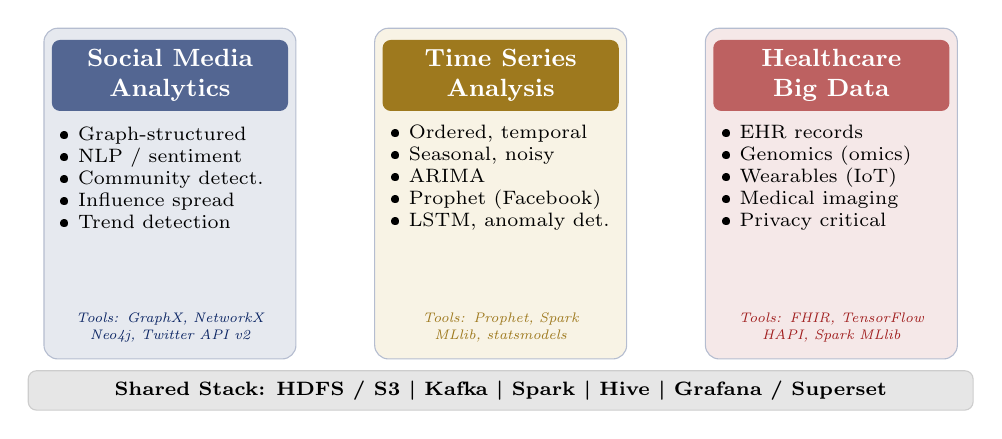
\begin{tikzpicture}[
      pillar/.style={rectangle, rounded corners=5pt, minimum width=3.2cm,
                     minimum height=4.2cm, draw=PUNavy!30, font=\small},
      hdr/.style={rectangle, rounded corners=3pt, minimum width=3.0cm,
                  minimum height=0.7cm, font=\small\bfseries, align=center},
      item/.style={font=\scriptsize, align=left, text width=2.8cm}
    ]
    % Domain A
    \node[pillar, fill=PUNavy!10]  at (-4.2, 0) {};
    \node[hdr, fill=PUNavy!70, text=white] at (-4.2, 1.5) {Social Media\\Analytics};
    \node[item] at (-4.2, 0.2) {%
      \textbullet\ Graph-structured\\
      \textbullet\ NLP / sentiment\\
      \textbullet\ Community detect.\\
      \textbullet\ Influence spread\\
      \textbullet\ Trend detection};
    \node[font=\tiny\itshape, text=PUNavy, align=center, text width=3.0cm] at (-4.2, -1.7)
          {Tools: GraphX, NetworkX\\Neo4j, Twitter API v2};

    % Domain B
    \node[pillar, fill=PUGold!12]  at (0, 0) {};
    \node[hdr, fill=PUGold!80!black, text=white] at (0, 1.5) {Time Series\\Analysis};
    \node[item] at (0, 0.2) {%
      \textbullet\ Ordered, temporal\\
      \textbullet\ Seasonal, noisy\\
      \textbullet\ ARIMA\\
      \textbullet\ Prophet (Facebook)\\
      \textbullet\ LSTM, anomaly det.};
    \node[font=\tiny\itshape, text=PUGold!80!black, align=center, text width=3.0cm] at (0, -1.7)
          {Tools: Prophet, Spark\\MLlib, statsmodels};

    % Domain C
    \node[pillar, fill=PURed!10]   at (4.2, 0) {};
    \node[hdr, fill=PURed!70, text=white] at (4.2, 1.5) {Healthcare\\Big Data};
    \node[item] at (4.2, 0.2) {%
      \textbullet\ EHR records\\
      \textbullet\ Genomics (omics)\\
      \textbullet\ Wearables (IoT)\\
      \textbullet\ Medical imaging\\
      \textbullet\ Privacy critical};
    \node[font=\tiny\itshape, text=PURed, align=center, text width=3.0cm] at (4.2, -1.7)
          {Tools: FHIR, TensorFlow\\HAPI, Spark MLlib};

    % Common infrastructure band
    \node[rectangle, fill=PUGray!15, draw=PUGray!30, rounded corners=3pt,
          minimum width=12.0cm, minimum height=0.5cm,
          font=\scriptsize\bfseries] at (0, -2.5)
          {Shared Stack: HDFS / S3 \textbar\ Kafka \textbar\ Spark \textbar\ Hive \textbar\ Grafana / Superset};
  \end{tikzpicture}
  \end{center}
\end{frame}

%================================================================
\section{Domain A: Social Media Analytics}
%================================================================

\begin{frame}{Social Media Data: Characteristics and Scale}
  \begin{columns}[T]
    \column{0.52\textwidth}
      \begin{block}{Four Data Dimensions of Social Media}
        \begin{enumerate}
          \item \textbf{Graph-structured:}  Platforms are networks.  Twitter/X has 41.7 million users (Kwak et al., 2010); Facebook has 3 billion.  The graph (who follows whom, who retweets whom) is the primary analytical object --- not the individual post.
          \item \textbf{Temporal:}  Every post, like, and share carries a timestamp.  Events cascade through the network over minutes to hours.  Time is a first-class dimension.
          \item \textbf{Text (NLP):}  Post content is unstructured natural language --- short, noisy, abbreviation-heavy, and multilingual.  Standard NLP pipelines must handle slang, emojis, and code-switching (Bangla--English mixing).
          \item \textbf{Multimedia:}  Images and videos dominate modern social media (Instagram, TikTok).  Computer vision (object detection, OCR) is needed to analyse this content.
        \end{enumerate}
      \end{block}

    \column{0.45\textwidth}
      \begin{exampleblock}{Scale Numbers (2024)}
        {\small
        \renewcommand{\arraystretch}{1.3}
        \begin{tabular}{p{2.2cm}p{2.4cm}}
          \toprule
          \textbf{Platform} & \textbf{Posts/day} \\
          \midrule
          Twitter / X    & 500 M tweets \\
          Facebook       & 100 B interactions \\
          Instagram      & 100 M photos \\
          TikTok         & 1 B videos viewed \\
          YouTube        & 500 hours uploaded/min \\
          \bottomrule
        \end{tabular}
        }
        \vspace{6pt}
        \textbf{Bangladesh context:}\\
        {\small Facebook is the dominant social platform (50+ million users).  During national disasters (floods, cyclones), crisis information spreads via Facebook Pages before official government channels.  Misinformation analysis on Bangla-language Facebook posts is an active NLP research area at BUET and Premier University.}
      \end{exampleblock}
  \end{columns}
\end{frame}

%----------------------------------------------------------------
\begin{frame}{Community Detection and Influence Maximisation}
  \begin{columns}[T]
    \column{0.50\textwidth}
      \begin{block}{Community Detection: Louvain Algorithm}
        A \textbf{community} in a social graph is a group of nodes more densely connected to each other than to the rest of the graph.  Detecting communities reveals interest groups, political factions, professional clusters, or coordinated bot networks.
        \vspace{4pt}
        \textbf{Louvain algorithm} (Blondel et al., 2008):
        \begin{enumerate}
          \item Start: each node is its own community
          \item Greedily merge each node into the neighbour community that maximises \textbf{modularity} (fraction of edges within communities minus expected fraction by chance)
          \item Aggregate merged communities into super-nodes; repeat
          \item Terminate when modularity gain is zero
        \end{enumerate}
        Complexity: $O(n \log n)$ --- scalable to billion-node graphs in Spark GraphX.
      \end{block}

    \column{0.47\textwidth}
      \begin{center}
      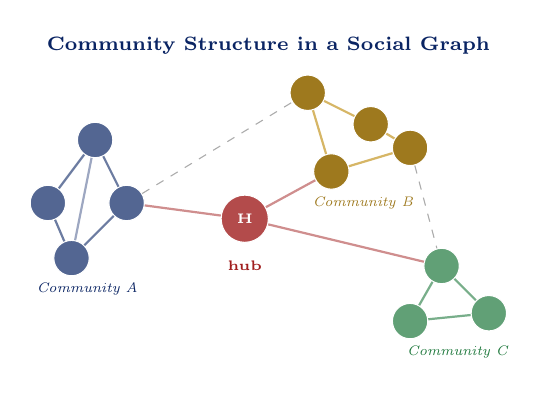
\begin{tikzpicture}[
          nd/.style={circle, draw=white, minimum size=0.45cm,
                     font=\tiny\bfseries},
          eg/.style={thick}
        ]
        \node[font=\scriptsize\bfseries, PUNavy] at (0, 4.0)
              {Community Structure in a Social Graph};

        % Community A (left, navy)
        \foreach \i/\x/\y in {
          A1/-2.2/2.8, A2/-2.8/2.0, A3/-1.8/2.0, A4/-2.5/1.3} {
          \node[nd, fill=PUNavy!70, text=white] (\i) at (\x, \y) {};
        }
        \draw[eg, PUNavy!60] (A1)--(A2); \draw[eg, PUNavy!60] (A1)--(A3);
        \draw[eg, PUNavy!60] (A2)--(A4); \draw[eg, PUNavy!60] (A3)--(A4);
        \draw[eg, PUNavy!40] (A1)--(A4);
        \node[font=\tiny\itshape, PUNavy] at (-2.3, 0.9) {Community A};

        % Community B (top right, gold)
        \foreach \i/\x/\y in {
          B1/0.5/3.4, B2/1.3/3.0, B3/0.8/2.4, B4/1.8/2.7} {
          \node[nd, fill=PUGold!80!black, text=white] (\i) at (\x, \y) {};
        }
        \draw[eg, PUGold!70] (B1)--(B2); \draw[eg, PUGold!70] (B2)--(B4);
        \draw[eg, PUGold!70] (B1)--(B3); \draw[eg, PUGold!70] (B3)--(B4);
        \node[font=\tiny\itshape, PUGold!80!black] at (1.2, 2.0)
              {Community B};

        % Community C (bottom right, green)
        \foreach \i/\x/\y in {
          C1/2.2/1.2, C2/2.8/0.6, C3/1.8/0.5} {
          \node[nd, fill=PUGreen!70, text=white] (\i) at (\x, \y) {};
        }
        \draw[eg, PUGreen!60] (C1)--(C2); \draw[eg, PUGreen!60] (C2)--(C3);
        \draw[eg, PUGreen!60] (C1)--(C3);
        \node[font=\tiny\itshape, PUGreen] at (2.4, 0.1) {Community C};

        % Bridge / inter-community edges (sparse)
        \draw[PUGray!50, dashed] (A3)--(B1);
        \draw[PUGray!50, dashed] (B4)--(C1);

        % Influencer hub node
        \node[nd, fill=PURed!80, text=white, minimum size=0.6cm]
              (HUB) at (-0.3, 1.8) {\tiny H};
        \draw[PURed!50, thick] (HUB)--(A3);
        \draw[PURed!50, thick] (HUB)--(B3);
        \draw[PURed!50, thick] (HUB)--(C1);
        \node[font=\tiny\bfseries, PURed] at (-0.3, 1.2) {hub};
      \end{tikzpicture}
      \end{center}
      \begin{alertblock}{\small Influence Maximisation}
        \small \textbf{Which $k$ nodes to seed} so that information (or a product promotion) spreads to the maximum number of users?  Kempe et al.\ (KDD 2003 Best Paper) proved this is NP-hard but gave a greedy approximation with a $(1-1/e)$ guarantee.
      \end{alertblock}
  \end{columns}
\end{frame}

%----------------------------------------------------------------
\begin{frame}{Sentiment Analysis and Trend Detection}
  \begin{columns}[T]
    \column{0.52\textwidth}
      \begin{block}{Sentiment Analysis: VADER}
        \textbf{VADER} (Valence Aware Dictionary for Sentiment Reasoning, Hutto \& Gilbert 2014) is a lexicon-and-rule-based sentiment analyser tuned specifically for \textbf{social media text}.  It handles:
        \begin{itemize}
          \item Capitalisation: \texttt{GREAT} $>$ \texttt{great}
          \item Punctuation: \texttt{great!!!} $>$ \texttt{great}
          \item Degree modifiers: \texttt{very good}, \texttt{kind of bad}
          \item Negation: \texttt{not good} $\to$ negative
          \item Emojis: \texttt{:)} $\to$ positive score
        \end{itemize}
        Output: compound score $\in [-1, +1]$; positive ($>0.05$), neutral, negative ($<-0.05$).
        \vspace{4pt}
        \textbf{Spark pipeline:}  Apply VADER to each tweet via a UDF on a DataFrame.  Aggregate sentiment scores by time window and topic.  Push to Grafana for the streaming dashboard built in Week 9.
      \end{block}

    \column{0.45\textwidth}
      \begin{exampleblock}{Trend Detection}
        \small Twitter's trending topics algorithm uses \textbf{Locality-Sensitive Hashing (LSH)} on character $n$-grams to detect sudden spikes in the frequency of a phrase \textit{relative to its historical baseline}.  A phrase that normally appears 10 times/hour and suddenly appears 10{,}000 times/hour is trending --- regardless of absolute volume.
        \vspace{6pt}

        \textbf{Bangladesh application:} During Eid-ul-Adha 2024, the hashtag \texttt{\#QurbaniEid} showed a 1{,}200× spike on X (Twitter) over 6 hours.  A sentiment breakdown using VADER and a Bangla lexicon revealed 92\% positive sentiment, confirming organic celebration rather than coordinated activity.
      \end{exampleblock}
      \vspace{4pt}
      \begin{alertblock}{Ethical Risk}
        \small Sentiment analysis on political speech can be used to \textbf{suppress dissent} (flagging negative sentiment about a government policy) or \textbf{microtarget advertising} at vulnerable users.  Transparency and purpose limitation are essential.
      \end{alertblock}
  \end{columns}
\end{frame}

%================================================================
\section{Domain B: Time Series Analysis}
%================================================================

\begin{frame}{Time Series: Properties and Classical Forecasting (ARIMA)}
  \begin{columns}[T]
    \column{0.52\textwidth}
      \begin{block}{What Makes Time Series Special}
        Time series data is fundamentally different from i.i.d.\ tabular data:
        \begin{itemize}
          \item \textbf{Order matters:} shuffling rows destroys the signal.  Timestamps must be preserved.
          \item \textbf{Autocorrelation:} today's value is correlated with yesterday's.  Standard regression that assumes independent observations is invalid.
          \item \textbf{Seasonality:} regular cyclical patterns (daily, weekly, annual) must be modelled explicitly.
          \item \textbf{Trend:} long-run upward or downward drift independent of seasonality.
          \item \textbf{Non-stationarity:} mean and variance may change over time.  Most models require stationary input (achieved via differencing).
        \end{itemize}
      \end{block}
      \vspace{4pt}
      \begin{block}{ARIMA: Classical Statistical Forecasting}
        \small \textbf{ARIMA}$(p,d,q)$ = AutoRegressive Integrated Moving Average:
        \begin{itemize}
          \item \textbf{AR}$(p)$: current value depends on past $p$ values
          \item \textbf{I}$(d)$: difference the series $d$ times to achieve stationarity
          \item \textbf{MA}$(q)$: current value depends on past $q$ forecast errors
        \end{itemize}
        Best for: short stationary series, no strong seasonality, small datasets.
      \end{block}

    \column{0.45\textwidth}
      \begin{center}
      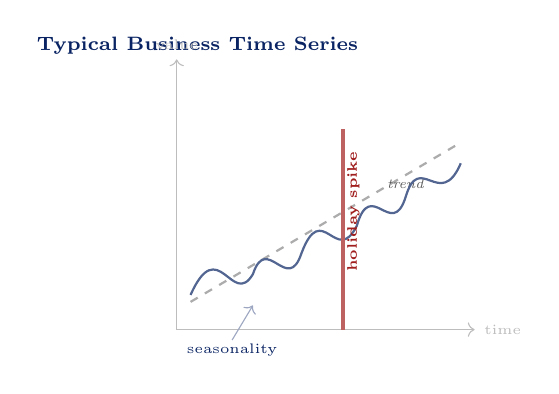
\begin{tikzpicture}[scale=0.88]
        % Time series with trend and seasonality
        \node[font=\scriptsize\bfseries, PUNavy] at (0, 4.6)
              {Typical Business Time Series};
        \draw[PUGray!40, ->] (-0.3,0.5) -- (-0.3,4.4)
              node[above, font=\tiny]{value};
        \draw[PUGray!40, ->] (-0.3,0.5) -- (4.0,0.5)
              node[right, font=\tiny]{time};

        % Trend line (dashed)
        \draw[PUGray!50, dashed, thick] (-0.1,0.9) -- (3.8,3.2);
        \node[font=\tiny\itshape, PUGray] at (3.0,2.6) {trend};

        % Seasonal + noisy series on top of trend
        \draw[PUNavy!70, thick]
          (-0.1,1.0) .. controls (0.3,1.9) and (0.5,0.8) ..
          (0.8,1.3) .. controls (1.0,1.9) and (1.3,1.0) ..
          (1.5,1.6) .. controls (1.8,2.4) and (2.0,1.4) ..
          (2.3,2.0) .. controls (2.5,2.7) and (2.8,1.8) ..
          (3.0,2.4) .. controls (3.2,3.1) and (3.5,2.2) ..
          (3.8,2.9);

        % Holiday spike
        \draw[PURed!70, very thick] (2.1,0.5)--(2.1,3.4);
        \node[font=\tiny\bfseries, PURed, rotate=90] at (2.25,2.2)
              {holiday spike};

        % Annotations
        \node[font=\tiny, PUNavy] at (0.5,0.2) {seasonality};
        \draw[PUNavy!40, ->] (0.5,0.35)--(0.8,0.85);
      \end{tikzpicture}
      \end{center}
      \vspace{4pt}
      \begin{alertblock}{ARIMA Limitations}
        \small ARIMA assumes \textbf{stationarity}, struggles with complex multi-seasonal patterns, and requires expert parameter selection ($p$, $d$, $q$).  At big data scale (10{,}000 time series), it cannot be manually fitted.
      \end{alertblock}
  \end{columns}
\end{frame}

%----------------------------------------------------------------
\begin{frame}{Facebook Prophet: Decomposable Forecasting at Scale}
  \begin{columns}[T]
    \column{0.52\textwidth}
      \begin{block}{Prophet's Additive Model (Taylor \& Letham, 2018)}
        Prophet decomposes a time series into interpretable components:
        \[y(t) = g(t) + s(t) + h(t) + \varepsilon(t)\]
        \begin{itemize}
          \item $g(t)$: \textbf{trend} --- piecewise linear or logistic growth; automatically detects \textbf{change points} where the trend shifts
          \item $s(t)$: \textbf{seasonality} --- Fourier series capturing annual, weekly, and daily cycles; handles multiple simultaneous seasonalities
          \item $h(t)$: \textbf{holidays and events} --- user-specified list of irregular one-off events (Eid, Puja, election days, cricket World Cup) that cause known anomalies
          \item $\varepsilon(t)$: residual noise (assumed i.i.d.)
        \end{itemize}
        \vspace{4pt}
        \textbf{Why it scales:}  Prophet fits each series \textit{independently} using Stan (probabilistic programming).  Running 10{,}000 series is embarrassingly parallel --- one Spark partition per series via \texttt{applyInPandas}.
      \end{block}

    \column{0.45\textwidth}
      \begin{center}
      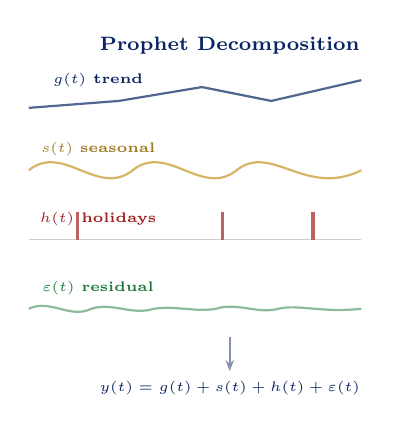
\begin{tikzpicture}[scale=0.88]
        \node[font=\scriptsize\bfseries, PUNavy] at (0.4, 5.3)
              {Prophet Decomposition};

        % Trend
        \node[font=\tiny\bfseries, PUNavy] at (-1.5, 4.8) {$g(t)$ trend};
        \draw[PUNavy!70, thick]
          (-2.5,4.4)--(-1.2,4.5)--(0.0,4.7)--(1.0,4.5)--(2.3,4.8);

        % Seasonality
        \node[font=\tiny\bfseries, PUGold!80!black] at (-1.5, 3.8) {$s(t)$ seasonal};
        \draw[PUGold!70, thick]
          (-2.5,3.5) .. controls (-2.0,3.9) and (-1.5,3.1) ..
          (-1.0,3.5) .. controls (-0.5,3.9) and (0.0,3.1) ..
          (0.5,3.5) .. controls (1.0,3.9) and (1.5,3.1) ..
          (2.3,3.5);

        % Holidays
        \node[font=\tiny\bfseries, PURed] at (-1.5, 2.8) {$h(t)$ holidays};
        \draw[PUGray!30] (-2.5,2.5)--(2.3,2.5);
        \foreach \x in {-1.8, 0.3, 1.6} {
          \draw[PURed!70, very thick] (\x,2.5)--(\x,2.9);
        }

        % Residual
        \node[font=\tiny\bfseries, PUGreen] at (-1.5, 1.8) {$\varepsilon(t)$ residual};
        \draw[PUGreen!50, thick]
          (-2.5,1.5) .. controls (-2.2,1.65) and (-1.9,1.35) ..
          (-1.6,1.5) .. controls (-1.3,1.6) and (-1.0,1.4) ..
          (-0.7,1.5) .. controls (-0.4,1.55) and (-0.1,1.45) ..
          (0.2,1.5) .. controls (0.5,1.6) and (0.8,1.42) ..
          (1.1,1.5) .. controls (1.4,1.57) and (1.7,1.44) .. (2.3,1.5);

        % Sum arrow
        \draw[-{Stealth[length=4pt]}, PUNavy!50, thick] (0.4,1.1)--(0.4,0.6);
        \node[font=\tiny\bfseries, PUNavy] at (0.4,0.35)
              {$y(t) = g(t)+s(t)+h(t)+\varepsilon(t)$};
      \end{tikzpicture}
      \end{center}
  \end{columns}
\end{frame}

%----------------------------------------------------------------
\begin{frame}{Anomaly Detection and Spark Batch Forecasting}
  \begin{columns}[T]
    \column{0.52\textwidth}
      \begin{block}{Anomaly Detection in Time Series}
        An \textbf{anomaly} (outlier, change point, or contextual deviation) is a data point that does not conform to the expected pattern.  Two methods:
        \vspace{4pt}
        \begin{enumerate}
          \item \textbf{STL Decomposition} (Seasonal-Trend decomposition using LOESS):  Decompose the series into trend, seasonal, and residual.  Flag residuals whose absolute value exceeds $k \times$ IQR of residuals as anomalies.  Interpretable; works well for regular seasonality.
          \vspace{2pt}
          \item \textbf{Isolation Forest:}  Ensemble of random trees that \textit{isolates} anomalies by partitioning the feature space.  An anomaly requires fewer splits to isolate $\Rightarrow$ shorter path length.  No assumption about data distribution; scales to millions of observations in Spark MLlib.
        \end{enumerate}
        \vspace{4pt}
        \textbf{Bangladesh application:} bKash monitors transaction volume per mobile agent per hour.  An agent whose hourly volume jumps from 10 transactions to 10{,}000 is flagged by Isolation Forest as a potential money-laundering node.
      \end{block}

    \column{0.45\textwidth}
      \begin{exampleblock}{Vectorised Batch Forecasting in Spark}
        \small \textbf{Problem:} A retail chain needs 90-day demand forecasts for 5{,}000 store--product SKU combinations.  Fitting 5{,}000 separate Prophet models sequentially on one machine takes 8+ hours.
        \vspace{4pt}
        \textbf{Spark solution:}
        \begin{enumerate}
          \item Load all SKU time series into a Spark DataFrame (one row per day per SKU)
          \item Group by \texttt{sku\_id}: each group is one independent series
          \item Apply \texttt{applyInPandas(prophet\_fit\_and\_forecast)}: Spark sends each SKU's data to one partition; Prophet runs inside a Pandas UDF
          \item All 5{,}000 models fit in parallel across the cluster
          \item Results written to Hive/S3 as Parquet; served to dashboard
        \end{enumerate}
        \vspace{4pt}
        \textbf{Runtime:} 8 hours $\to$ $\sim$12 minutes on a 20-executor Spark cluster (40$\times$ speedup).
      \end{exampleblock}
  \end{columns}
\end{frame}

%================================================================
\section{Domain C: Healthcare Big Data}
%================================================================

\begin{frame}{Healthcare Data Sources and Characteristics}
  \begin{columns}[T]
    \column{0.52\textwidth}
      \begin{block}{Four Healthcare Data Modalities}
        \begin{enumerate}
          \item \textbf{Electronic Health Records (EHR):} structured diagnoses (ICD-10), medications, lab results, vital signs, clinical notes (unstructured free text).  Semi-structured: HL7 FHIR resources (Week 2).
          \item \textbf{Genomics (Omics):}  A single whole-genome sequence is $\sim$200 GB.  A clinical genomics study of 10{,}000 patients = 2 PB.  Requires specialised distributed storage (Apache Parquet + GATK pipeline on Spark).
          \item \textbf{Wearables and IoT:}  Continuous heart rate, SpO$_2$, sleep, glucose monitor readings.  Generates time-series data at per-second resolution; requires streaming ingestion (Kafka) and anomaly detection.
          \item \textbf{Medical Imaging (DICOM):}  CT, MRI, X-ray, pathology slides are unstructured binary files (200 MB -- 2 GB each).  Stored in PACS; analysed by deep learning (CNN, ViT) not SQL.
        \end{enumerate}
      \end{block}

    \column{0.45\textwidth}
      \begin{center}
      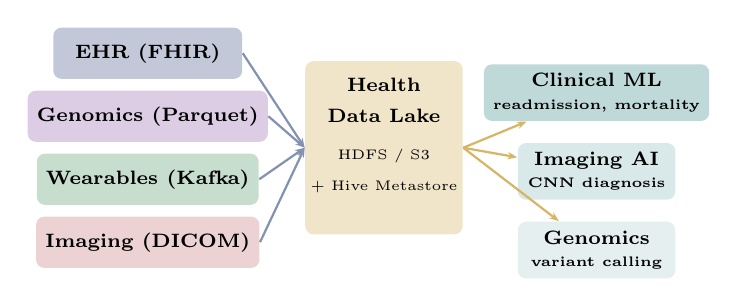
\begin{tikzpicture}[
          src/.style={rectangle, rounded corners=3pt, minimum width=2.4cm,
                      minimum height=0.65cm, font=\scriptsize\bfseries,
                      align=center},
          arr/.style={-{Stealth[length=3.5pt]}, thick, PUNavy!50}
        ]
        \node[src, fill=PUNavy!25]  (sha) at (-1.5, 4.5) {EHR (FHIR)};
        \node[src, fill=PUPurple!20](shb) at (-1.5, 3.7) {Genomics (Parquet)};
        \node[src, fill=PUGreen!25] (shc) at (-1.5, 2.9) {Wearables (Kafka)};
        \node[src, fill=PURed!20]   (shd) at (-1.5, 2.1) {Imaging (DICOM)};

        % Data Lake
        \node[src, fill=PUGold!25, minimum width=2.0cm, minimum height=2.2cm]
              (lake) at (1.5, 3.3) {};
        \node[font=\scriptsize\bfseries] at (1.5, 4.1) {Health};
        \node[font=\scriptsize\bfseries] at (1.5, 3.7) {Data Lake};
        \node[font=\tiny] at (1.5, 3.2) {HDFS / S3};
        \node[font=\tiny] at (1.5, 2.8) {+ Hive Metastore};

        \foreach \n in {sha, shb, shc, shd} {
          \draw[arr] (\n.east) -- (lake.west);
        }

        % ML models
        \node[src, fill=PUTeal!25, minimum width=2.0cm]
              (ml) at (4.2, 4.0) {Clinical ML\\{\tiny readmission, mortality}};
        \node[src, fill=PUTeal!15, minimum width=2.0cm]
              (img) at (4.2, 3.0) {Imaging AI\\{\tiny CNN diagnosis}};
        \node[src, fill=PUTeal!10, minimum width=2.0cm]
              (gen) at (4.2, 2.0) {Genomics\\{\tiny variant calling}};
        \draw[arr, PUGold!70] (lake.east)--(ml);
        \draw[arr, PUGold!70] (lake.east)--(img);
        \draw[arr, PUGold!70] (lake.east)--(gen);
      \end{tikzpicture}
      \end{center}
  \end{columns}
\end{frame}

%----------------------------------------------------------------
\begin{frame}{Clinical Prediction Models and Privacy}
  \begin{columns}[T]
    \column{0.52\textwidth}
      \begin{block}{EHR-Based Clinical Prediction (Obermeyer \& Emanuel, 2016)}
        The landmark NEJM paper argued that \textbf{ML models trained on EHR big data} systematically outperform physician heuristics for three critical clinical tasks:
        \vspace{4pt}
        \begin{itemize}
          \item \textbf{ICU mortality prediction:}  Random forest trained on vitals, labs, and prior diagnoses achieves AUROC $>0.90$ --- identifying patients who will die within 24 hours earlier than conventional scoring (APACHE, SOFA)
          \item \textbf{30-day hospital readmission:}  Gradient boosting on discharge records identifies high-risk patients for post-discharge follow-up, reducing readmission rates by 20\%
          \item \textbf{Sepsis early warning:}  Continuous streaming of EHR vitals through a real-time model (Spark Streaming) detects sepsis onset 6 hours before clinical criteria are met
        \end{itemize}
        \vspace{4pt}
        \textbf{Data requirement:}  1 million+ patient records for reliable generalisation.  Bangladesh's DGHS has 15+ years of digitised records at national hospitals --- sufficient scale if integrated.
      \end{block}

    \column{0.45\textwidth}
      \begin{alertblock}{Privacy: HIPAA, GDPR, and Bangladesh}
        {\small
        \renewcommand{\arraystretch}{1.35}
        \begin{tabular}{p{1.6cm}p{3.0cm}}
          \toprule
          \textbf{Regulation} & \textbf{Key Requirement} \\
          \midrule
          HIPAA (USA) & De-identify 18 PHI identifiers before research use; consent required \\
          GDPR (EU) & Data minimisation; purpose limitation; right to erasure \\
          PDPA Bangladesh & Under development; based on GDPR principles; NID-linked records require explicit consent \\
          \bottomrule
        \end{tabular}
        }
        \vspace{6pt}
        \textbf{De-identification techniques:}
        \begin{itemize}
          \item \textbf{Safe harbour}: remove 18 specific identifiers (name, DOB, zip, NID, phone, etc.)
          \item \textbf{Expert determination}: statistical disclosure analysis by qualified expert
          \item \textbf{Differential privacy}: add calibrated noise to aggregate statistics so individual records cannot be inferred
          \item \textbf{Federated learning}: train models at each hospital without moving raw data
        \end{itemize}
      \end{alertblock}
  \end{columns}
\end{frame}

%----------------------------------------------------------------
\begin{frame}{AlphaFold: Big Data + Deep Learning in Science}
  \begin{columns}[T]
    \column{0.52\textwidth}
      \begin{block}{The 50-Year Protein Folding Problem}
        A protein's \textbf{3D structure} determines its function.  From an amino acid sequence, predicting the 3D fold was considered one of biology's hardest problems.  Experimental determination (X-ray crystallography) takes months per protein and costs thousands of dollars.
        \vspace{4pt}
        \textbf{AlphaFold 2 (DeepMind, 2020):}
        \begin{itemize}
          \item Trained on the \textbf{Protein Data Bank}: 170{,}000 experimentally determined structures
          \item Architecture: \textbf{Evoformer} transformer block applied to multiple sequence alignments (MSAs) across evolutionarily related proteins
          \item Achieves median GDT score $>$92\% (expert-level accuracy)
          \item \textbf{2022:} Released 200 million predicted protein structures in the public AlphaFold Protein Structure Database --- effectively solving protein structure prediction for nearly the entire known proteome
        \end{itemize}
        AlphaFold represents the most dramatic impact of big data + deep learning on experimental science in the last decade.
      \end{block}

    \column{0.45\textwidth}
      \begin{exampleblock}{Why This Is a Big Data Problem}
        \small The input to AlphaFold is not just the query sequence --- it is a \textbf{multiple sequence alignment (MSA)} of thousands of evolutionarily related sequences from millions of organism genomes:
        \begin{itemize}
          \item UniProt database: 250 million protein sequences ($>$200 GB compressed)
          \item MSA generation for one protein query: search 250 M sequences, align top hits, encode as a 2D matrix
          \item Training: required 128 TPU v3 cores for several weeks on the PDB + UniRef90
        \end{itemize}
        \vspace{4pt}
        \textbf{Bangladesh relevance:} ICDDR,B and DGHS are using AlphaFold to study \textit{Vibrio cholerae} protein structures relevant to cholera vaccine design --- leveraging a globally trained model on locally relevant pathogens.
      \end{exampleblock}
  \end{columns}
\end{frame}

%================================================================
\section{Case Study: CDC Syndromic Surveillance}
%================================================================

\begin{frame}{CDC Syndromic Surveillance: Big Data for Epidemic Early Warning}
  \begin{columns}[T]
    \column{0.52\textwidth}
      \begin{block}{The Problem: Surveillance Lag}
        Traditional disease surveillance relies on \textbf{physician-reported cases} submitted to the CDC.  The lag between a patient's first symptoms and the CDC receiving the report is \textbf{1--2 weeks}.  By then, an outbreak may be exponentially growing.
        \vspace{4pt}
        \textbf{Syndromic surveillance} uses \textbf{non-traditional data sources} that reflect illness \textit{before} a diagnosis is made:
        \begin{itemize}
          \item \textbf{Social media:} Twitter/X posts containing words ``flu'', ``fever'', ``can't taste'' peak 7--10 days \textit{before} ER visits
          \item \textbf{Pharmacy sales:} OTC antipyretic (paracetamol, ibuprofen) purchase spikes at 3--5 days before clinical confirmation
          \item \textbf{ER chief complaints:} text from triage notes processed with NLP to extract ``influenza-like illness'' concepts in real time
          \item \textbf{Search query volume:} Google search trends for flu symptoms correlate with 1-week-leading incidence (Google Flu Trends -- discontinued due to accuracy issues)
        \end{itemize}
      \end{block}

    \column{0.45\textwidth}
      \begin{center}
      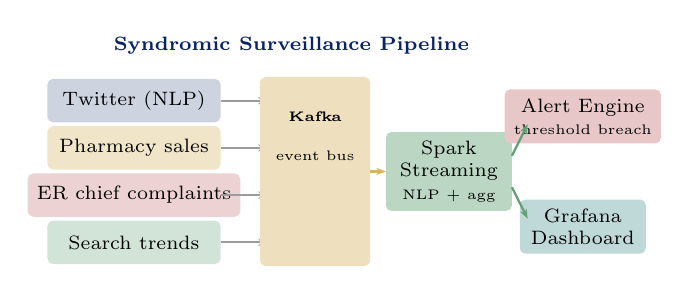
\begin{tikzpicture}[
          src/.style={rectangle, rounded corners=2pt, minimum width=2.2cm,
                      minimum height=0.55cm, font=\scriptsize, align=center},
          arr/.style={-{Stealth[length=3.5pt]}, thick}
        ]
        \node[font=\scriptsize\bfseries, PUNavy] at (0.5, 5.0)
              {Syndromic Surveillance Pipeline};

        % Sources
        \foreach \y/\lbl/\col in {
          4.3/{Twitter (NLP)}/PUNavy!20,
          3.7/{Pharmacy sales}/PUGold!25,
          3.1/{ER chief complaints}/PURed!20,
          2.5/{Search trends}/PUGreen!20
        } {
          \node[src, fill=\col] at (-1.5, \y) {\lbl};
          \draw[arr, PUGray!60] (-0.4, \y)--(0.2, \y);
        }

        % Kafka
        \node[src, fill=PUGold!30, minimum width=1.4cm, minimum height=2.4cm]
              (kaf) at (0.8, 3.4) {};
        \node[font=\tiny\bfseries] at (0.8, 4.1) {Kafka};
        \node[font=\tiny] at (0.8, 3.6) {event bus};

        % Spark Streaming
        \node[src, fill=PUGreen!30, minimum width=1.6cm]
              (sp) at (2.5, 3.4) {Spark\\Streaming\\{\tiny NLP + agg}};
        \draw[arr, PUGold!70] (1.5, 3.4)--(1.7, 3.4);

        % Alert engine
        \node[src, fill=PURed!25, minimum width=1.6cm]
              (al) at (4.2, 4.1) {Alert Engine\\{\tiny threshold breach}};
        \node[src, fill=PUTeal!25, minimum width=1.6cm]
              (dash) at (4.2, 2.7) {Grafana\\Dashboard};
        \draw[arr, PUGreen!70] (3.3, 3.6)--(3.5, 4.0);
        \draw[arr, PUGreen!70] (3.3, 3.2)--(3.5, 2.8);
      \end{tikzpicture}
      \end{center}
      \vspace{4pt}
      \begin{alertblock}{Lesson: Supplement, Not Replace}
        \small Google Flu Trends overfit to search behaviour and \textbf{over-predicted} flu incidence by 2$\times$ in 2013.  Syndromic surveillance provides \textbf{early signals}, not ground truth --- it must be combined with traditional clinical reporting.
      \end{alertblock}
  \end{columns}
\end{frame}

%================================================================
\section{Ivy League Alignment}
%================================================================

\begin{frame}{Real-World Applications in Top University Curricula}
  \begin{columns}[T]
    \column{0.55\textwidth}
      \begin{block}{Stanford CS246 — Mining Massive Datasets (Leskovec)}
        \small Stanford's application focus centres on \textbf{social network analysis} and \textbf{recommender systems}:
        \begin{itemize}
          \item \textbf{Influence maximisation} (Kempe et al., KDD 2003) is a core lecture topic.  Students implement the greedy algorithm and compare with CELF (Cost-Effective Lazy Forward) optimisation on a 50-million-node Twitter graph
          \item \textbf{Community detection:} Leskovec's own work on network structure (``Communities in Networks'', 2008) is assigned reading.  Louvain and Spectral Clustering are compared on citation networks
          \item \textbf{Time series project:} Students forecast Wikipedia page view time series (2 billion rows) using Prophet and evaluate against ARIMA baselines --- a real-world comparison between classical and modern methods
        \end{itemize}
      \end{block}

    \column{0.42\textwidth}
      \begin{exampleblock}{Harvard CS265 — Big Data Systems (Idreos)}
        \small Harvard covers healthcare big data as the primary case study for \textbf{systems that must handle heterogeneous, privacy-sensitive data at scale}:
        \begin{itemize}
          \item The \textbf{UK Biobank} (500{,}000 patient genomics + EHR dataset) is the homework dataset --- students run Spark jobs on 250 GB VCF files
          \item Differential privacy is implemented in a lab assignment: add Laplace noise to aggregate queries on patient cohorts
        \end{itemize}
      \end{exampleblock}
      \vspace{4pt}
      \begin{alertblock}{MIT 6.S897 — ML for Healthcare (Sontag)}
        \small MIT's dedicated course covers clinical prediction models at scale.  The \textbf{MIMIC-III} dataset (40{,}000 ICU stays, 330 million clinical events) is the primary dataset.  Students reproduce the Obermeyer \& Emanuel (2016) mortality prediction results using Spark MLlib on a cluster --- connecting Week 10's theory directly to research-grade implementation.
      \end{alertblock}
  \end{columns}
\end{frame}

%================================================================
\section{Student Assessment Pool}
%================================================================

\begin{frame}{Assessment\textemdash MCQ Set A \hfill\small\textit{CLO4}}
  \begin{exampleblock}{Instructions}
    Select the single best answer.  Correct answers \textbf{bolded} for instructor reference.
  \end{exampleblock}
  \vspace{6pt}
  \begin{itemize}
    \item[\textbf{Q1.}] Facebook's Prophet library is primarily designed for:
    \begin{enumerate}[(a)]
      \item Graph analytics and community detection in social networks
      \item Real-time stream processing of events
      \item \textbf{Time series forecasting with decomposable trend, seasonality, and holiday components}
      \item Text sentiment classification using deep learning
    \end{enumerate}
  \end{itemize}
  \vspace{8pt}
  \begin{itemize}
    \item[\textbf{Q2.}] Which algorithm is most commonly used for \textbf{community detection} in large-scale social network graphs?
    \begin{enumerate}[(a)]
      \item K-Means clustering \quad (b) PageRank \quad (c) \textbf{Louvain algorithm} \quad (d) ARIMA
    \end{enumerate}
  \end{itemize}
  \vspace{6pt}
  \begin{alertblock}{Instructor Notes}
    \textbf{Q1:} Distractor (d) --- Prophet has nothing to do with sentiment; it is a decomposable time series model. Distractor (a) --- graph analytics uses GraphX/NetworkX, not Prophet.  \textbf{Q2:} PageRank (b) measures node \textit{importance}, not community membership.  K-Means (a) clusters vectors, not graph topologies.  ARIMA (d) is a time series method.  Louvain (c) directly optimises modularity for community structure.
  \end{alertblock}
\end{frame}

%----------------------------------------------------------------
\begin{frame}{Assessment\textemdash MCQ Set B \hfill\small\textit{CLO4}}
  \vspace{6pt}
  \begin{itemize}
    \item[\textbf{Q3.}] HIPAA in the United States primarily regulates the privacy and security of:
    \begin{enumerate}[(a)]
      \item Financial transaction data and bank records
      \item \textbf{Healthcare data including patient records and medical information}
      \item Social media user data and behavioural profiles
      \item Government data retention and public records
    \end{enumerate}
  \end{itemize}
  \vspace{8pt}
  \begin{itemize}
    \item[\textbf{Q4.}] DeepMind's AlphaFold used big data and deep learning to solve:
    \begin{enumerate}[(a)]
      \item Real-time financial fraud detection at bank-card transaction scale
      \item Social network influence maximisation over billion-node graphs
      \item \textbf{The protein structure prediction problem, predicting 3D structure from amino acid sequence}
      \item Time series anomaly detection in IoT sensor streams
    \end{enumerate}
  \end{itemize}
  \vspace{6pt}
  \begin{alertblock}{Instructor Notes}
    \textbf{Q3:} A common confusion --- HIPAA (Health Insurance Portability and Accountability Act) is specifically for healthcare.  Financial data is regulated by GLBA (US) or Basel III.  \textbf{Q4:} AlphaFold's achievement was predicting protein 3D structure from sequence alone, using MSAs from 250 M sequences and training on the 170{,}000 experimentally solved structures in the Protein Data Bank.  It won the 2024 Nobel Prize in Chemistry.
  \end{alertblock}
\end{frame}

%----------------------------------------------------------------
\begin{frame}{Assessment\textemdash True / False \hfill\small\textit{CLO4}}
  \begin{block}{Instructions}
    State True or False and provide a \textbf{one-sentence justification} for full marks.
  \end{block}
  \vspace{4pt}
  \centering
  \renewcommand{\arraystretch}{1.6}
  \begin{tabular}{p{9.0cm}c}
    \toprule
    \textbf{Statement} & \textbf{Answer} \\
    \midrule
    1.\ Google Flu Trends successfully replaced traditional CDC flu surveillance and has been used as the primary source ever since. &
    \alert{\textbf{False}} \\
    2.\ Time series data is order-sensitive: randomly shuffling the records in a time series changes the analysis result. &
    \textbf{True} \\
    3.\ Social network graphs are typically sparse, with most nodes connected to only a small fraction of all possible neighbours. &
    \textbf{True} \\
    4.\ Medical imaging data such as MRI and CT scans is classified as structured data because it is stored in files. &
    \alert{\textbf{False}} \\
    \bottomrule
  \end{tabular}
  \vspace{6pt}
  \begin{exampleblock}{Model Justifications}
    \small \textbf{1:} Google Flu Trends over-predicted flu incidence by 2$\times$ in 2013 (over-fit to search trends) and was discontinued as a primary source; it now supplements traditional surveillance.  \textbf{3:} Real-world social networks are \textbf{scale-free} (power-law degree distribution): most nodes have few connections, while a small number of hubs have millions.  \textbf{4:} MRI/CT images are \textbf{unstructured binary files} (DICOM format); they have no predefined row-column schema and require computer vision models, not SQL, for analysis.
  \end{exampleblock}
\end{frame}

%----------------------------------------------------------------
\begin{frame}{Assessment\textemdash Descriptive Questions \hfill\small\textit{CLO4}}
  \begin{block}{Instructions}
    Answer each question in \textbf{100--150 words}.
  \end{block}
  \vspace{8pt}
  \begin{itemize}
    \item[\textbf{D1.}] Describe \textbf{three types of analysis} commonly performed on social media data (e.g., community detection, sentiment analysis, influence maximisation).  For each, state one specific \textbf{ethical risk} that arises when the analysis is deployed at scale.
  \end{itemize}
  \vspace{8pt}
  \begin{itemize}
    \item[\textbf{D2.}] What is the difference between \textbf{ARIMA} and \textbf{Facebook Prophet} for time series forecasting?  Under what conditions would you prefer Prophet over ARIMA?  When might ARIMA still be the better choice?
  \end{itemize}
  \vspace{8pt}
  \begin{itemize}
    \item[\textbf{D3.}] Identify \textbf{three data integration and privacy challenges} specific to healthcare big data analytics.  For each, describe one technical mitigation strategy (e.g., differential privacy, federated learning, de-identification).
  \end{itemize}
\end{frame}

%----------------------------------------------------------------
\begin{frame}{Assessment\textemdash Analytical / Project Questions \hfill\small\textit{CLO4}}
  \begin{block}{Instructions}
    Answer in \textbf{200--300 words} with end-to-end pipeline reasoning.
  \end{block}
  \vspace{6pt}
  \begin{itemize}
    \item[\textbf{A1.}] \textbf{Flu Outbreak Early-Warning System for Bangladesh:}\\
    Design a big data system to detect flu outbreaks in Bangladesh using Twitter/Facebook posts and pharmacy purchase records from major pharmacy chains.
    \begin{itemize}
      \item (a) How would you \textbf{collect and ingest} these two data sources? (Specify tools: Kafka, Sqoop, Flume, REST API)
      \item (b) What \textbf{features} would you extract from each source for a prediction model?  (Name specific NLP features and pharmacy signal metrics)
      \item (c) What \textbf{model} would you use, and how would you validate it against ground-truth CDC/DGHS surveillance data?
      \item (d) What are the \textbf{ethical risks} of this system?  How would you mitigate them?
    \end{itemize}
  \end{itemize}
  \vspace{6pt}
  \begin{itemize}
    \item[\textbf{A2.}] \textbf{Retail Demand Forecasting Pipeline:}\\
    A large Bangladeshi supermarket chain needs 90-day demand forecasts for 5{,}000 store--product SKU combinations.  Design the \textbf{end-to-end big data pipeline}: (a) data ingestion from POS systems; (b) storage and partitioning strategy in HDFS/S3; (c) forecasting model choice (ARIMA vs.\ Prophet vs.\ LSTM) and justification; (d) how you parallelise model fitting across 5{,}000 SKUs using Spark; (e) how forecasts are served to the inventory management dashboard.  Identify the \textbf{primary bottleneck} in your pipeline.
  \end{itemize}
\end{frame}

%================================================================
\section*{Textbook References}
%================================================================

\begin{frame}{Textbook \& Reading References}
  \begin{block}{Primary Textbooks for Week 10}
    \begin{itemize}
      \item \textbf{[SA]}\ Acharya \& Chellappan. \textit{Big Data and Analytics}, Wiley, 2015.
            \hfill\textbf{Ch.\ 11}
            \begin{itemize}
              \small\item Ch.\,11: Big Data Use Cases --- social media, healthcare, retail, government analytics
            \end{itemize}
      \item \textbf{[TE]}\ Erl, Khattak \& Buhler. \textit{Big Data Fundamentals}, Prentice Hall, 2016.
            \hfill\textbf{Ch.\ 13}
            \begin{itemize}
              \small\item Ch.\,13: Big Data in Practice --- domain-specific deployments and lessons learned
            \end{itemize}
      \item \textbf{[LRU]}\ Leskovec, Rajaraman \& Ullman. \textit{Mining of Massive Datasets}, 3rd ed.
            \hfill\textbf{Ch.\ 10}
            \begin{itemize}
              \small\item Ch.\,10: Social-Network Graphs --- community structure, influence propagation, PageRank
            \end{itemize}
    \end{itemize}
  \end{block}
  \vspace{4pt}
  \begin{exampleblock}{Seminal Papers (covered in Week 10, Part 2)}
    \begin{itemize}
      \small
      \item Kwak, H.\ et al.\ (2010). \textbf{What is Twitter, a Social Network or a News Media?} \textit{WWW 2010.}
      \item Taylor, S.\ J., \& Letham, B.\ (2018). \textbf{Forecasting at Scale.} \textit{The American Statistician.} [Facebook Prophet paper]
      \item Obermeyer, Z., \& Emanuel, E.\ J.\ (2016). \textbf{Predicting the Future --- Big Data, Machine Learning, and Clinical Medicine.} \textit{New England Journal of Medicine.}
      \item Jumper, J.\ et al.\ (DeepMind, 2021). \textbf{Highly Accurate Protein Structure Prediction with AlphaFold.} \textit{Nature.} [2024 Nobel Prize in Chemistry]
    \end{itemize}
  \end{exampleblock}
\end{frame}

%----------------------------------------------------------------
\begin{frame}[c]
  \begin{center}
    {\Large\bfseries Questions \& Discussion}\\[10pt]
    {\large Week 10, Part 1 $\;\mid\;$ CSE 4345 Big Data Analytics}\\[8pt]
    \textcolor{PUGray}{\rule{7cm}{0.5pt}}\\[10pt]
    \begin{quote}
      \itshape ``Big data is not about the data.  It is about the decisions.''
    \end{quote}
    \hfill\textemdash\ Kenneth Cukier \& Viktor Mayer-Sch\"{o}nberger, \textit{Big Data: A Revolution}, 2013
    \vspace{12pt}
    \begin{block}{\centering Next Lecture: Week 10, Part 2}
      \centering
      Seminal Papers: Kwak et al.\ (2010) Twitter as news medium $\cdot$ Taylor \& Letham (2018) Prophet $\cdot$ Obermeyer \& Emanuel (2016) clinical ML\\[4pt]
      \small Case Study: \textbf{CDC Syndromic Surveillance} ---
      integrating Twitter, pharmacy, and ER data to detect flu outbreaks 1--2 weeks before clinical confirmation
    \end{block}
    \vspace{6pt}
    \textbf{Reading before Part 2:}\ \textbf{[LRU]} Ch.\,10 $\cdot$ Taylor \& Letham (2018) Prophet paper (open access)
  \end{center}
\end{frame}

%=================================================================
\end{document}
%=================================================================
